\documentclass{article}

% if you need to pass options to natbib, use, e.g.:
% \PassOptionsToPackage{numbers, compress}{natbib}
% before loading nips_2016
%
% to avoid loading the natbib package, add option nonatbib:
% \usepackage[nonatbib]{nips_2016}

\usepackage[final,nonatbib]{nips_2016}

% to compile a camera-ready version, add the [final] option, e.g.:
% \usepackage[final]{nips_2016}

\usepackage[utf8]{inputenc} % allow utf-8 input
\usepackage[T1]{fontenc}    % use 8-bit T1 fonts
\usepackage{hyperref}       % hyperlinks
\usepackage{url}            % simple URL typesetting
\usepackage{booktabs}       % professional-quality tables
\usepackage{amsfonts}       % blackboard math symbols
\usepackage{nicefrac}       % compact symbols for 1/2, etc.
\usepackage{microtype}      % microtypography
\usepackage{amsmath}
\usepackage{tikz}
\usetikzlibrary{positioning}
\usetikzlibrary{shapes.geometric}
\usetikzlibrary{calc}

\tikzset{
  multiplexer/.style={
    draw,
    trapezium,
    shape border uses incircle, 
    shape border rotate=270,
    minimum size=18pt
  }
}

\bibliographystyle{ieeetr}

\title{Project Proposal}

% The \author macro works with any number of authors. There are two
% commands used to separate the names and addresses of multiple
% authors: \And and \AND.
%
% Using \And between authors leaves it to LaTeX to determine where to
% break the lines. Using \AND forces a line break at that point. So,
% if LaTeX puts 3 of 4 authors names on the first line, and the last
% on the second line, try using \AND instead of \And before the third
% author name.

\author{
    Kyle~Daruwalla \\
    Department of Electrical and Computer Engineering \\
    University of Wisconsin -- Madison \\
    \texttt{daruwalla@wisc.edu} \\
    \And
    Akhil~Sundararajun \\
    Department of Electrical and Computer Engineering \\
    University of Wisconsin -- Madison \\
    \texttt{asundararaja@wisc.edu} \\
}

\begin{document}

\maketitle

% Each section (including abstract) has its own .tex file
% The name of the .tex file corresponds to the section title
% e.x. The subsection in the Introduction on FPGAs is called
%      intro-fpga.tex
% \input{filename} is equivalent to pasting in the raw text
% from filename.tex.
% Try to edit the filename.tex files and not proposal.tex.
% This avoids conflicts most of the time.

\section{Introduction}
\textit{Include brief information on setting up the CNN problem.}
Testing

\subsection{Field-Programmable Gate Arrays}
\textit{Include brief information on FPGAs.}

\section{Problem Definition}
Convolutional neural networks are optimized for classification of structured data, such as images, and map input data into labels through successive representation layers.  Each layer abstracts information about the layer previous through a nonlinear activation function.  
To find a classifier that abstracts patterns in input data, we would like to minimize the empirical risk on the training data, given $m$ training example-label pairs $\{(x_i,y_i)\}_{i=1}^m$.
\begin{equation}
	\min_{f\in F}\sum_{i=1}^n \mathcal{L}(f(x_i);y_i)
	\label{eq:erm}
\end{equation}
where $\mathcal{L}$ is some loss function assigns a value related to the discrepancy between the label generated by the model $f$ and the true label.  SGD is used to solve the ERM, but its serial nature motivates the investigation of methods that achieve speedup.


\section{Proposed Implementation}
In order to perform an effective comparison between software implementations of CNNs and hardware implementations, we propose using TensorFlow, Amazon EC2, and Xilinx FPGAs. TensorFlow will be used to implement various software implementations of a given CNN structure for ImageNet. These CNN implementations will be trained and tested on Amazon EC2. A hardware implementation of the CNN will be created for Xilinx FPGAs in Vivado. Simulations will be performed to verify its functionality, and it will be deployed on a physical FPGA to test its timing characteristics and accuracy.
\subsection{TensorFlow on EC2}
The first experiment will be to study training performance of the ImageNet dataset on Amazon EC2, which will serve as a baseline for a traditional single-machine CPU setting.  We propose to use TensorFlow, an open-source, python-based machine learning package released by Google in November 2015 \cite{tensorflow}.  In addition, using packages in TensorFlow, we will study GPU acceleration on Amazon EC2.  Due to TensorFlow’s distributed execution capability, we also propose to train CNNs using the {\sc{Hogwild!}} algorithm.  Since SGD is inherently serial, our FPGA implementation targets lowering cost per iteration.  This can be compared to {\sc{Hogwild!}}, which is a parallelized approach to achieving speedup.  Due to the variety of structural and parameter design choices typical in building a CNN, we also propose to examine several CNN architectures in combination with the different hardware platforms considered in this project.  Different activation functions including sign, ReLU, and sigmoid also will be explored.

\subsection{Neural Networks on FPGAs}
Each filter in the CNN will be modeled as a \textit{unit-neuron} on the FPGA (shown in Figure \ref{fig:unit-neuron}). During the compute phase, the selector signal $s$, will feed the current patch $(x_0, x_1, x_2, x_3, x_4)$ into the unit-neuron. A weight register file will hold the current weights, $(w_0, w_1, w_2, w_3, w_4)$. The activation function, $\sigma$, will be approximated using a lookup table if it is not piecewise linear. The output $f$ will store a single pixel of output for a given filter.
\begin{figure}[hb]
	\centering
	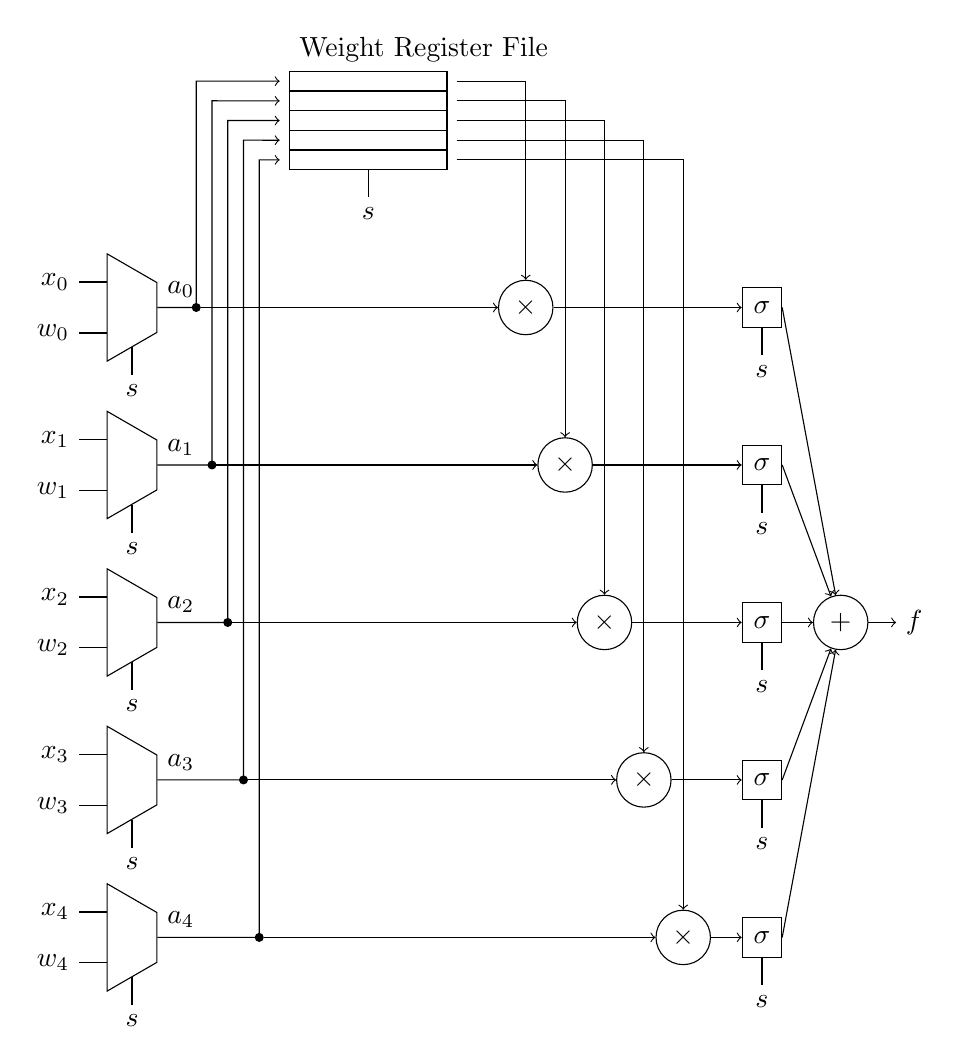
\begin{tikzpicture}
		\foreach \i in {0, ..., 4} {
			\node[multiplexer] (mux\i) at (0, -2*\i) {};
			\draw (mux\i.north west) --++ (-10pt, 0) node [left] {$x_\i$};
			\draw (mux\i.south west) --++ (-10pt, 0) node [left] {$w_\i$};
			\draw (mux\i.south) --++ (0, -10pt) node [below] {$s$};
		}

		\draw (2, 3) node[above right] {Weight Register File} rectangle (4, 1.75);
		\draw (3, 1.75) --++ (0, -10pt) node[below] {$s$};
		\foreach \i in {0, ..., 4} {
			\draw ($(2, {2.75-0.25*\i})$) node[above] (wrf\i) {} --++ (2, 0) node[above] (wrf\i-out) {};
			\draw [->] (mux\i.top side) node [above right] {$a_\i$} --++ (14pt, 0) --++ (0.2*\i, 0) node[circle, fill, draw, inner sep=-1pt] (junc\i) {} --++ ($(0, 2.875+1.75*\i)$) -- (wrf\i);
		}

		\foreach \i in {0, ..., 4} {
			\node[circle, draw] (mul\i) at ($(5+0.5*\i, -2*\i)$) {$\times$};
			\draw [->] (junc\i) -- (mul\i.west);
			\draw [->] (wrf\i-out) --++ ($(1+0.5*\i, 0)$) -- (mul\i.north);
		}

		\node[circle, draw] (sum) at (9, -4) {$+$};

		\foreach \i in {0, ..., 4} {
			\node[rectangle, minimum height=0.5cm, minimum width=0.5cm, draw] (sigma\i) at ($(8, -2*\i)$) {$\sigma$};
			\draw [->] (mul\i.east) -- (sigma\i.west);
			\draw [->] (sigma\i.east) -- (sum);
			\draw (sigma\i.south) --++ (0, -10pt) node[below] {$s$};
		}

		\draw [->] (sum.east) --++ (10pt, 0) node[right] {$f$};
	\end{tikzpicture}
	\caption{A unit-neuron implementation for an FPGA with a filter size of 5}
	\label{fig:unit-neuron}
\end{figure}

A controller will adjust $(x_0, x_1, x_2, x_3, x_4)$ so that it corresponds to the current patch being evaluated. After the compute phase is complete, it will update the $(w_0, w_1, w_2, w_3, w_4)$ values and drive $s$ high so that the weight register file can be updated. There will be latching (not shown in Figure \ref{fig:unit-neuron}) on the output values of the filters so that they can be held while the weights are updated.

The potential for speedup comes from parallelizing the filter operation, using faster fixed-point computation units, and approximation of the activation function.

\section{Proposed Analysis}
\textit{Talk about analysis that we are targeting.}

\nocite{*}
\bibliography{references}

\end{document}
